
\documentclass[preprint,12pt]{elsarticle}

\usepackage[spanish]{babel}
\usepackage{amssymb}
\usepackage{graphicx}
\usepackage{lineno}
\usepackage[utf8]{inputenc}
\usepackage{url}
\usepackage{natbib} 
\usepackage{amsmath} 
\usepackage{amssymb} 

\begin{document}
	
	\begin{frontmatter}

		\title{\huge Gestores de BD NoSQL}
		
		\author{Aponte Roldán, Sigfredo              		(xxxxxxxxxx))}
		\author{Gonzales Cave, Angel Gabriel              	(2017057861))} %%cambiar
		\author{Pacora Silva, Jorge Carlos         		(xxxxxxxxxx))} %%cambiar
		\author{Quispe Mamani, José Luis             		(xxxxxxxxxx))} %%cambiar 
		\address{Tacna, Perú}
		
%% ABSTRACT --------------------------------------------------------------------------------------------------------------------

		\begin{abstract}
		
EDITAR

		\end{abstract}

%% ----------------------------------------------------------------------------------------------------------------------------------

	\end{frontmatter}

%% RESUMEN ---------------------------------------------------------------------------------------------------------------------

	\section{Resumen}

EDITAR

%% ----------------------------------------------------------------------------------------------------------------------------------


%% INTRODUCION ----------------------------------------------------------------------------------------------------------------

\section{Introducción} 

EDITAR

\begin{itemize}
\item A
\item B
\item C


\end{itemize}

%% ----------------------------------------------------------------------------------------------------------------------------------


%% MARCO TEÓRICO ------------------------------------------------------------------------------------------------------------

\section{Marco Teórico}

%% PRIMERA SUBSECCION 

\subsection {\textbf{A}}

\subsubsection{\textbf{A.1}}

EDITAR \cite{SQLne}  %% EJEMPLO DE COMO CITAR UNA REFERENCIA EN UN PÁRRAFO

\subsubsection{\textbf{A.2}}


\subsection {\textbf{Base de datos NoSQL orientadas a Documentos}}
Una base de datos orientada a documentos está diseñada para gestionar información orientada a documentos o datos semiestructurados. Tienen un grado de complejidad y flexibilidad superior a las bases de datos clave – valor. \newline
A diferencia de las conocidas bases de datos relacionales con su definición de “tabla”, los sistemas documentales están diseñados entorno a la definición abstracta de un “documento”. Un documento es la unidad principal de almacenamiento de este tipo de base de datos, y toda la información que aquí se almacena, se hace en formato de documento. \newline

Este tipo de Base de Datos NoSQL almacena la información como un documento, generalmente utilizando para ello una estructura simple como JSON o XML y donde se utiliza una clave única para cada registro. Este tipo de implementación permite, además de realizar búsquedas por clave – valor, realizar consultas más avanzadas sobre el contenido del documento.

\subsubsection{\textbf{Ventajas}}
\begin{itemize}

\item Almacenar y recuperar todos los datos relacionados como una sola unidad puede entregar ventajas enormes en el rendimiento y la escalabilidad.
\item Los gestores no tienen que hacer operaciones complejas como las uniones para encontrar los datos que normalmente están relacionados, ya que todo se encuentra en un mismo lugar.

\end{itemize}

\subsection {\textbf{MongoDB}}
MongoDB es una base de datos NoSQL Open Source orientada a documentos y ha sido diseñada con la idea de que fuera fácil tanto desarrollar para ella como de ser administrada. Un documento es una estructura de datos compuesta de pares de campos y valores. Además, estos objetos son muy similares a lo que serían objetos en notación JSON.\newline
Utilizar documentos tiene ciertas ventajas:
\begin{itemize}

\item Los documentos son tipos de datos nativos en muchos lenguajes de programación.
\item Los documentos embebidos y los arrays minimizan la necesidad de realizar joins muy pesados.
\item Tener un esquema dinámico es la base del polimorfismo.

\end{itemize}
\subsubsection{\textbf{Características generales}}
\begin{itemize}
\item 
\textbf{Indexado}\newline
MongoDB soporta índices secundarios, permitiendo una buena aceleración en muchas querys, pudiendo indexar cualquier campo de la base de datos.
\item 
\textbf{Agregación}\newline
MongoDB viene con muchas funciones predefinidas que facilitan en gran medida el tratamiento de las colecciones almacenadas.
\item
\textbf{Replicación y Balanceo de Carga}\newline
MongoDB utiliza un sistema de replicación empleando la arquitectura maestro – esclavo con el resto de máquinas. Además, hace uso de un tipo de particionado horizontal llamado sharding. Estas dos herramientas de escalado hacen de mongo una herramienta poderosa cuando se trata de crecer mucho en poco tiempo.

Mientras que la replicación busca realizar copias de los datos, repartirlos por nuevos hosts, permitiendo ofrecer alta disponibilidad, balanceo de carga y copias automáticas de seguridad, el sharding busca particionar esas tablas que, previsiblemente, se van haciendo más grandes y cada vez son más costosas de replicar.
\end{itemize}


\begin{figure}[htb]
	\begin{center}
		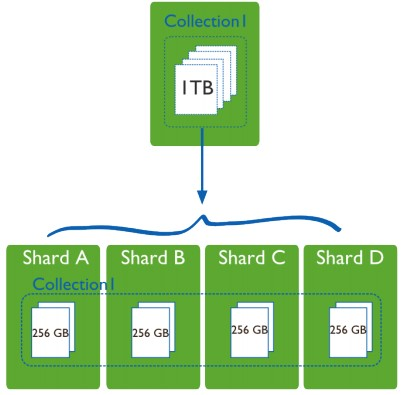
\includegraphics[width=6cm]{./IMAGENES/img01} %%EJEMPLO PARA INCLUIR IMAGEN
	\end{center}
\end{figure}

\subsubsection{\textbf{A.3}}

EDITAR

\begin{itemize}

\item x
\item y
\item z

\end{itemize}

%% SEGUNDA SUBSECCION

\subsection{\textbf{B}}

\subsubsection{\textbf{B.1}}

EDITAR

\subsubsection{\textbf{B.2}}	

EDITAR

\subsubsection{\textbf{B.3}}	

EDITAR


%% ----------------------------------------------------------------------------------------------------------------------------------


%% ANÁLISIS ( APLICACIÓN ) ---------------------------------------------------------------------------------------------------

\section{Análisis (Aplicación)}

EDITAR

%% ----------------------------------------------------------------------------------------------------------------------------------


%% CONCLUSIONES ---------------------------------------------------------------------------------------------------------------

\section{Conclusiones}

\begin{itemize}

\item Conclusion 1 : \\ A

\item Conclusion 2 : \\ B

\item Conclusion 3 : \\ C

\end{itemize}

%% ----------------------------------------------------------------------------------------------------------------------------------

%%  REFERENCIAS BIBLIOGRÁFICAS ------------------------------------------------------------------------------------------
	
	\newpage
	
	\bibliographystyle{apalike} 	%ESTILO
	\bibliography{BIBLIOGRAFIA}	 
	
	
\end{document}
